\documentclass[tikz,border=10pt]{standalone}
\usepackage{tikz}
\usepackage{pgfplots}
\pgfplotsset{compat=1.17}
\usetikzlibrary{calc,positioning,decorations.pathmorphing,arrows.meta,fadings,shapes.geometric}

\definecolor{coreC}{HTML}{2C5F8A}
\definecolor{shellC}{HTML}{5BA897}
\definecolor{ligC}{HTML}{C8783C}
\definecolor{edgeC}{HTML}{B0413E}
\definecolor{bulkC}{HTML}{3A3A4A}
\definecolor{accent}{HTML}{6A4C93}

\begin{document}

% ============================================================
% FIG 1 : Core-shell cross section
% ============================================================
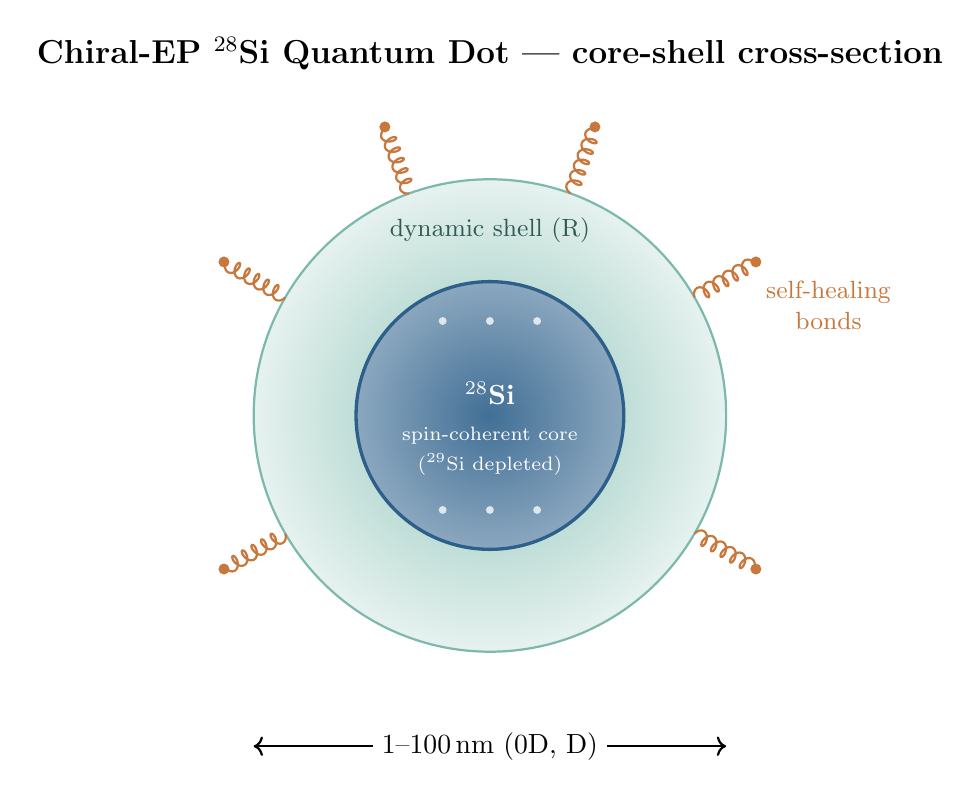
\begin{tikzpicture}[scale=1.0]
  \node at (0,4.6) {\large\bfseries Chiral-EP $^{28}$Si Quantum Dot — core-shell cross-section};

  % dynamic shell
  \shade[shading=radial,inner color=shellC!70,outer color=shellC!15]
        (0,0) circle (3.0);
  \draw[shellC!80,thick] (0,0) circle (3.0);
  % core
  \shade[shading=radial,inner color=coreC!90,outer color=coreC!55]
        (0,0) circle (1.7);
  \draw[coreC,very thick] (0,0) circle (1.7);

  % lattice dots in core (isotopically pure 28Si)
  \foreach \x in {-1.2,-0.6,0,0.6,1.2}{
    \foreach \y in {-1.2,-0.6,0,0.6,1.2}{
      \pgfmathsetmacro{\r}{sqrt(\x*\x+\y*\y)}
      \pgfmathsetmacro{\ay}{abs(\y)}
      \ifdim \r pt<1.55pt \ifdim \ay pt>0.75pt \fill[white!85!coreC] (\x,\y) circle (0.05); \fi\fi
    }}

  % dynamic reversible bonds on shell (decorative wavy ligands, sides/top only)
  \foreach \a in {30,70,110,150,210,330}{
    \draw[ligC,thick,decorate,decoration={coil,aspect=0.6,segment length=4pt,amplitude=2.5pt}]
      (\a:3.0) -- (\a:3.9);
    \fill[ligC] (\a:3.9) circle (0.07);
  }

  % labels
  \node[white] at (0,0.28) {\bfseries $^{28}$Si};
  \node[white,font=\scriptsize] at (0,-0.25) {spin-coherent core};
  \node[white,font=\scriptsize] at (0,-0.62) {($^{29}$Si depleted)};
  \node[shellC!55!black,font=\small] at (0,2.35) {dynamic shell (R)};
  \node[ligC,font=\small,align=center] at (4.3,1.4) {self-healing\\bonds};

  % size scale bar
  \draw[<->,thick] (-3.0,-4.2) -- (3.0,-4.2) node[midway,fill=white]{$1$–$100$\,nm (0D, D)};
\end{tikzpicture}

% ============================================================
% FIG 2 : 12-primitive type wheel
% ============================================================
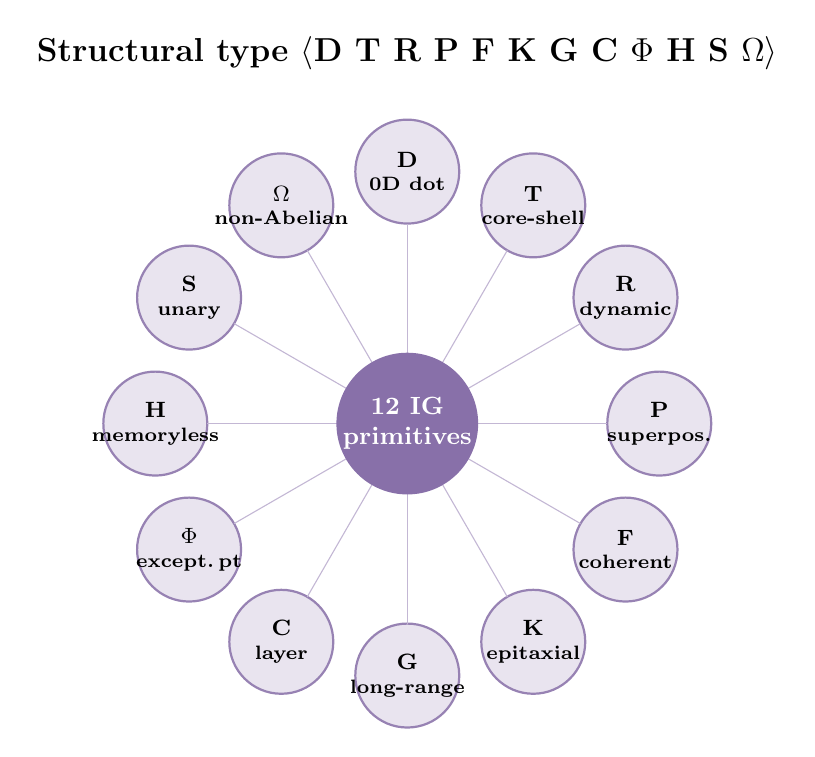
\begin{tikzpicture}[scale=1.0]
  \node at (0,4.7) {\large\bfseries Structural type $\langle$D T R P F K G C $\Phi$ H S $\Omega\rangle$};
  \def\R{3.2}
  \foreach \fam/\desc/\i in {%
      D/0D dot/0, T/core-shell/1, R/dynamic/2, P/superpos./3,
      F/coherent/4, K/epitaxial/5, G/long-range/6, C/layer/7,
      {$\Phi$}/except.\,pt/8, H/memoryless/9, S/unary/10, {$\Omega$}/non-Abelian/11}{
    \pgfmathsetmacro{\ang}{90-\i*30}
    \fill[accent!15] (\ang:\R) circle (0.66);
    \draw[accent!70,thick] (\ang:\R) circle (0.66);
    \node[font=\footnotesize\bfseries,align=center] at (\ang:\R) {\fam\\[-1pt]{\scriptsize\desc}};
    \draw[accent!40] (0,0) -- (\ang:{\R-0.66});
  }
  % center
  \fill[accent!80] (0,0) circle (0.9);
  \node[white,font=\small\bfseries,align=center] at (0,0) {12 IG\\primitives};
\end{tikzpicture}

% ============================================================
% FIG 3 : Exceptional-point sqrt(eps) response
% ============================================================
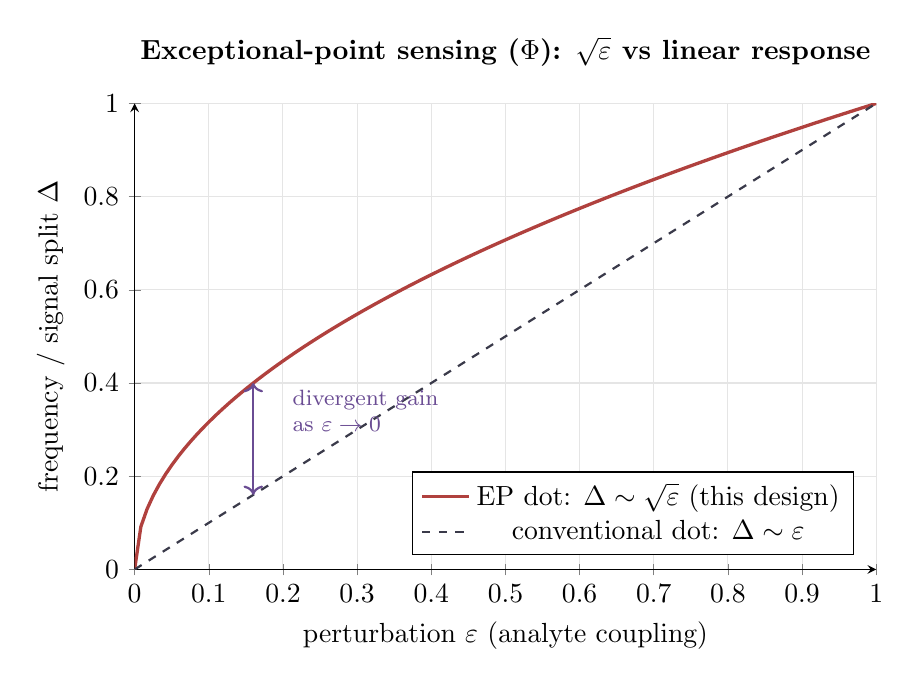
\begin{tikzpicture}
  \begin{axis}[
      width=11cm,height=7.5cm,
      title={\bfseries Exceptional-point sensing ($\Phi$): $\sqrt{\varepsilon}$ vs linear response},
      xlabel={perturbation $\varepsilon$ (analyte coupling)},
      ylabel={frequency / signal split $\Delta$},
      domain=0:1,samples=120,
      legend pos=south east,
      grid=both,grid style={gray!20},
      axis lines=left,
      title style={yshift=4pt}]
    \addplot[edgeC,very thick] {sqrt(x)};
    \addlegendentry{EP dot: $\Delta\sim\sqrt{\varepsilon}$ (this design)}
    \addplot[bulkC,thick,dashed] {x};
    \addlegendentry{conventional dot: $\Delta\sim\varepsilon$}
    % gap-between-curves annotation
    \draw[<->,accent,thick] (axis cs:0.16,0.16) -- (axis cs:0.16,0.40);
    \node[accent,right,font=\footnotesize,align=left]
      at (axis cs:0.20,0.34) {divergent gain\\as $\varepsilon\to0$};
  \end{axis}
\end{tikzpicture}

% ============================================================
% FIG 4 : Non-Abelian topological edge states
% ============================================================
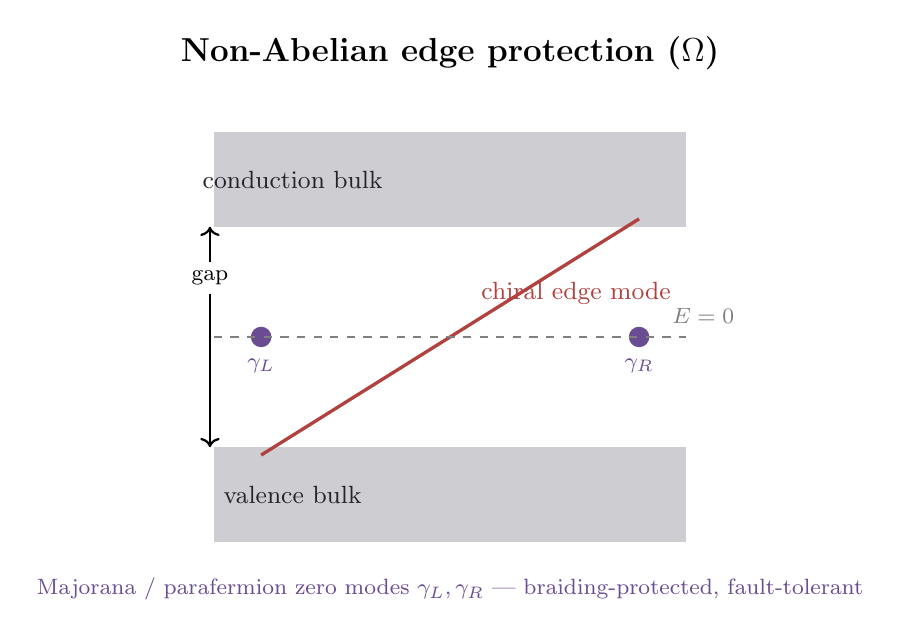
\begin{tikzpicture}[scale=1.0]
  \node at (0,3.6) {\large\bfseries Non-Abelian edge protection ($\Omega$)};

  % bulk bands
  \fill[bulkC!25] (-3,1.4) rectangle (3,2.6);
  \fill[bulkC!25] (-3,-2.6) rectangle (3,-1.4);
  \node[bulkC!60!black] at (-2.0,2.0) {\small conduction bulk};
  \node[bulkC!60!black] at (-2.0,-2.0) {\small valence bulk};

  % gap
  \draw[<->,thick] (-3.05,-1.4) -- (-3.05,1.4);
  \node[fill=white,font=\footnotesize] at (-3.05,0.75) {gap};

  % topological edge crossing (chiral mode)
  \draw[edgeC,very thick] (-2.4,-1.5) .. controls (0,0) .. (2.4,1.5);
  \node[edgeC] at (1.6,0.55) {\small chiral edge mode};

  % Majorana zero modes
  \fill[accent] (-2.4,0) circle (0.13);
  \fill[accent] (2.4,0) circle (0.13);
  \node[accent,below,font=\footnotesize] at (-2.4,-0.15) {$\gamma_L$};
  \node[accent,below,font=\footnotesize] at (2.4,-0.15) {$\gamma_R$};
  \node[accent,align=center,font=\footnotesize] at (0,-3.2)
    {Majorana / parafermion zero modes $\gamma_L,\gamma_R$ — braiding-protected, fault-tolerant};

  % zero energy line
  \draw[dashed,gray] (-3,0) -- (3.0,0);
  \node[gray,font=\footnotesize,above right] at (2.7,0.05) {$E=0$};
\end{tikzpicture}

\end{document}
